%--------------------------------------------------------%
% Figures
%--------------------------------------------------------%

%!TEX root = ../main.tex

%--------------------------------------------------------%
% DOCUMENT CLASS
%--------------------------------------------------------%

  % Change "letterpaper" to "a4" if you use a4 paper size
  \documentclass[letterpaper,12pt]{article}

%--------------------------------------------------------%
% TITLE SECTION
%--------------------------------------------------------%

  %Abstract
  \usepackage{abstract} % Allows abstract customization
  % Set the "Abstract" text to bold
  \renewcommand{\abstractnamefont}{\normalfont\bfseries}
  % Set the abstract itself to small italic text
  \renewcommand{\abstracttextfont}{\normalfont\small\itshape}

  %Title
  \usepackage{titlesec} % Allows customization of titles

  %Authors
  \usepackage{authblk} % For multiple authors

  %Date
  \usepackage{datetime} % allows for including today's date
  % These two lines creates a new date format ``Month day(th), year''
  \newdateformat{usvardate}{
  \monthname[\THEMONTH] \ordinal{DAY}, \THEYEAR}

%--------------------------------------------------------%
% HEADERS & FOOTERS
%--------------------------------------------------------%

  %Footnotes
  % \usepackage[bottom]{footmisc} % Makes footnotes stick to bottom of the page

  %Headers from page 2 on
  % \usepackage{fancyhdr}
  \pagestyle{plain}
  % \fancyheadoffset{0cm}
%   \setlength{\headheight}{15pt}

%--------------------------------------------------------%
% MACROS
%--------------------------------------------------------%

  % Define keywords macro command
  \providecommand{\keywords}[1]{\textbf{\textit{Keywords---}} #1}

%--------------------------------------------------------%
% MATH SUPPORT
%--------------------------------------------------------%

  % The amssymb package provides various useful mathematical symbols
  \usepackage{amssymb}
  % The amsthm package provides extended theorem environments
  \usepackage{amsthm}
  % The newtxmath package provides additional math symbol support
  % in Times New Roman symbols, etc.
  \usepackage{newtxmath}
  \usepackage{mathtools}
  \usepackage{blkarray, bigstrut}

%--------------------------------------------------------%
% FONTS
%--------------------------------------------------------%

  \usepackage{microtype} % Slightly tweak font spacing for aesthetics
  \usepackage[utf8]{inputenc}
  \usepackage{newtxtext} % Makes default font Adobe Times New Roman

%--------------------------------------------------------%
% LINES
%--------------------------------------------------------%

  % Spacing
  \usepackage{setspace} % See \doublespacing command at the top of content.tex
  % Numbering
  \usepackage{lineno} 	% See \linenumbers at the top of content.tex
  \usepackage[table,x11names]{xcolor}
  % Lists
  \usepackage{enumitem}
  \setlist{nosep}
  \setlist[itemize]{leftmargin=*}

%--------------------------------------------------------%
% MARGINS
%--------------------------------------------------------%

  %NOTE: All spaces in this template are in inches, because it is
  % formatted for letterpaper (8.5 x 11 inch) paper. If you use a4
  % paper, choose different sizes in millimeters or centimeters.
  \usepackage[top=1.5in, bottom=1.5in, left=1in, right=1in]{geometry}

%--------------------------------------------------------%
% COMMENTS
%--------------------------------------------------------%

  % \usepackage[colorinlistoftodos]{todonotes} % allows margin comments
  % See examples in content.tex, and here for manual:
  % http://www.ctan.org/pkg/todonotes
  \usepackage{soul} % allows for highlighting


%--------------------------------------------------------%
% ACRONYMS
%--------------------------------------------------------%

  \usepackage[nohyperlinks,nolist]{acronym} % Managing acronyms

%--------------------------------------------------------%
% GRAPHICS
%--------------------------------------------------------%

  \usepackage{graphicx,caption} % More advanced figure inclusion
  \graphicspath{{figures/}} % Set the default folder for images
  \usepackage{float} % For specifying table/figure locations, i.e. [ht!]

  % The printlen command allows the user to print the exact text width or height.
  % This is useful, when trying to create graphics (outside of LaTeX, of course)
  % with the optimal dimensions. See here for usage: http://www.ctan.org/pkg/printlen
  \usepackage{printlen}

  \usepackage[section]{placeins} % Used to ensure that figures do not go into the next section

%--------------------------------------------------------%
% TABLES
%--------------------------------------------------------%

  \usepackage{longtable} % For long tables that span multiple pages
  \newcommand{\sym}[1]{\rlap{#1}}% For symbols like *** in tables
  \usepackage{tabularx} % Allows advanced table features
  \newcolumntype{L}[1]{>{\raggedright\arraybackslash}p{#1}}
  \newcolumntype{C}[1]{>{\centering\arraybackslash}p{#1}}
  \newcolumntype{R}[1]{>{\raggedleft\arraybackslash}p{#1}}
  \usepackage{relsize} % Allows precise adjustment of font size,
  %useful for fitting tables to page width
  \usepackage{multirow}
  %for horizontal tables
  \usepackage{lscape}

%--------------------------------------------------------%
% REFERENCES
%--------------------------------------------------------%

  \usepackage{hyperref} % For hyperlinks in the PDF
  \usepackage{csquotes}
  \usepackage[style=nature,url=false,backend=biber,sorting=none]{biblatex}
  \bibliography{references/references.bib}


% \titleformat{\subsection}[runin]{}{}{}{}[]


\title{ \huge Microbial Interaction Database pipeline - Figures draft \#2 }
\author{DK, GB, ZH, CD, KK, DS}
\date{\today}

\begin{document}

\maketitle

\begin{figure}[h]
  \centering
  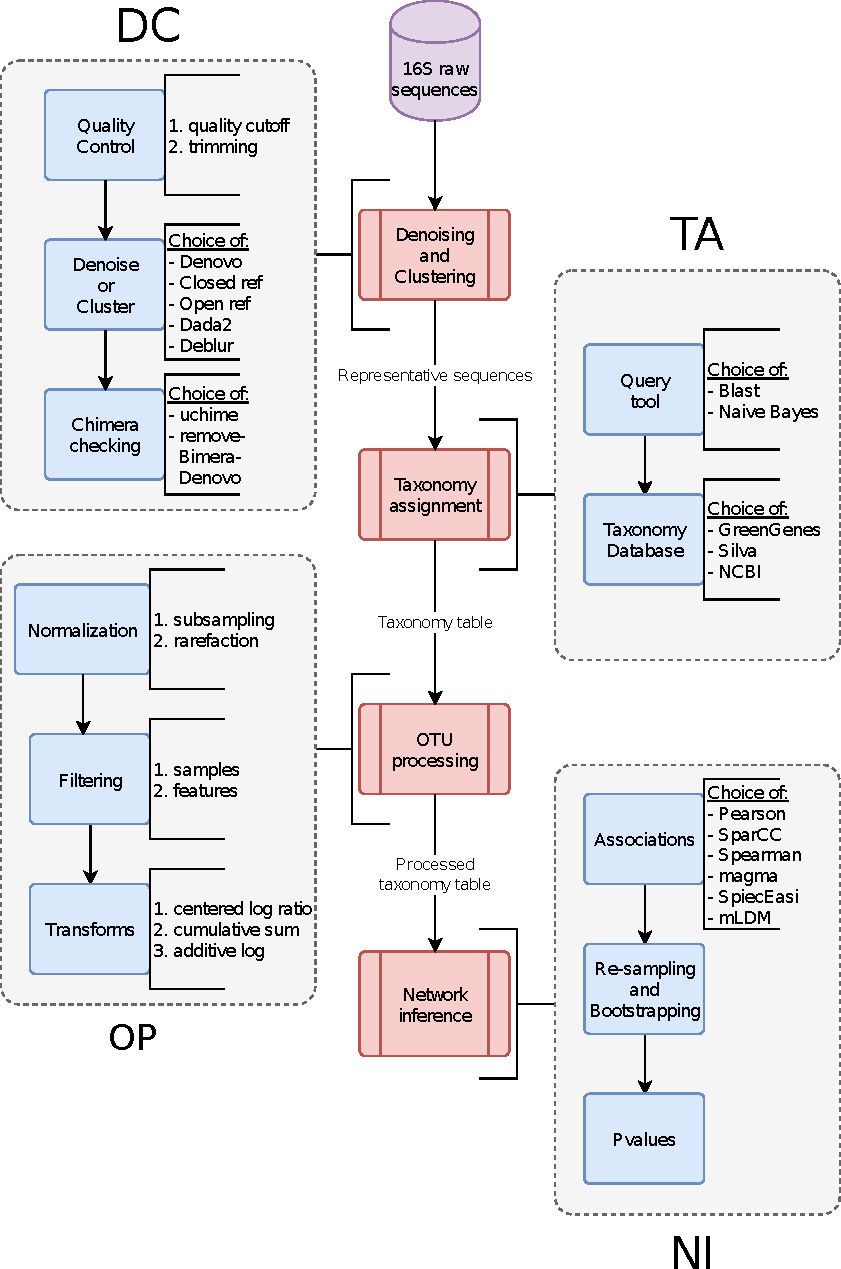
\includegraphics[width=\linewidth]{figure1.pdf}
  \caption{
    \textbf{The workflow of the microbial co-occurrence analysis pipeline}.
    The processes can be grouped into four major steps: \textbf{(A)} denoising and clustering, \textbf{(B)} taxonomy assignment, \textbf{(C)} OTU/ESV processing, and \textbf{(D)} network inference.
    Each step incorporates several processes, each of which in turn have several alternate algorithms for the same task (indicated by the text to the right of the blue boxes).
    \textbf{(E)} shows the average variances in the final networks contributed by each of the four groups over all the test datasets
  }
  \label{fig:main_figure}
\end{figure}

\begin{figure}[h]
  \centering
  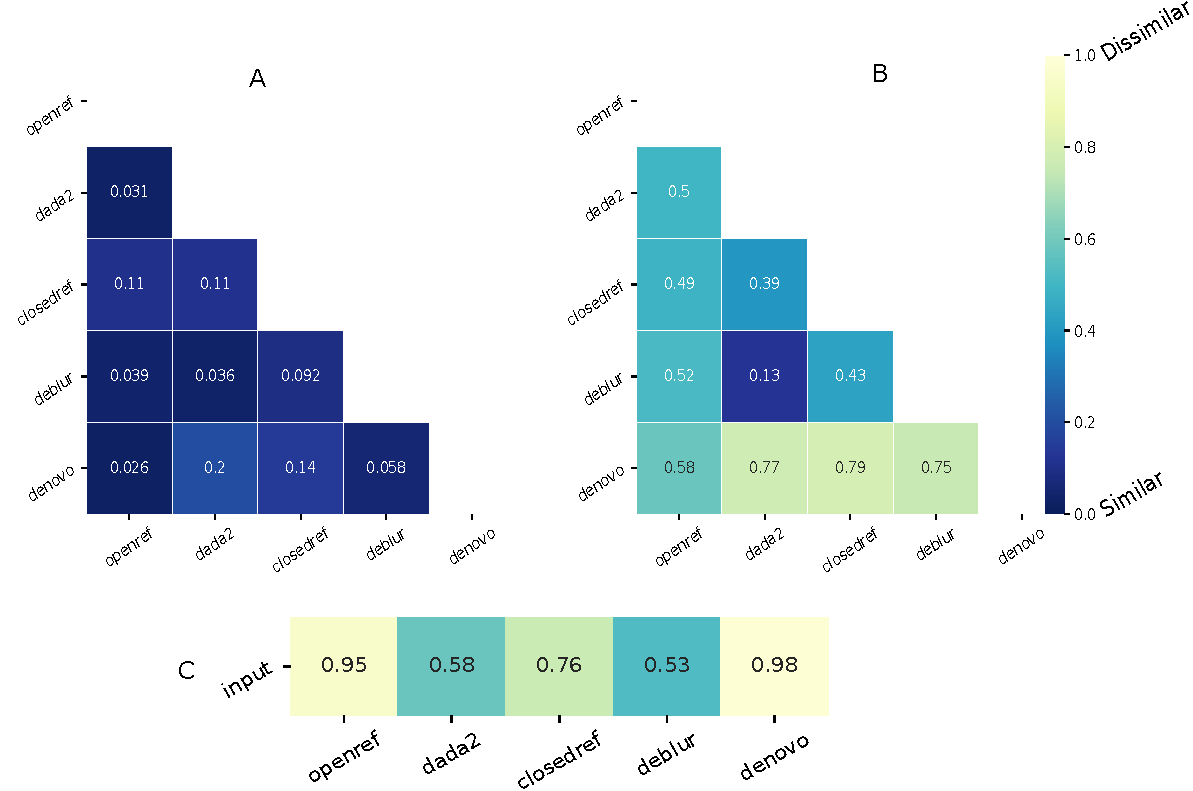
\includegraphics[width=\linewidth]{figure2.pdf}
  \caption{
    \textbf{Comparison of representative sequences generated by the various denoising and clustering algorithms used in the workflow.}
    \textbf{(A)} The average weighted UniFrac distance between the representative sequences,
    \textbf{(B)} The average unweighted UniFrac distance,
    \textbf{(C)} The distributions of the average unweighted UniFrac distance between original sequence profile and calculated profile in mock datasets (this will be replaced with a violoin plot)
  }
  \label{fig:figure2}
\end{figure}

\begin{figure}[h]
  \centering
  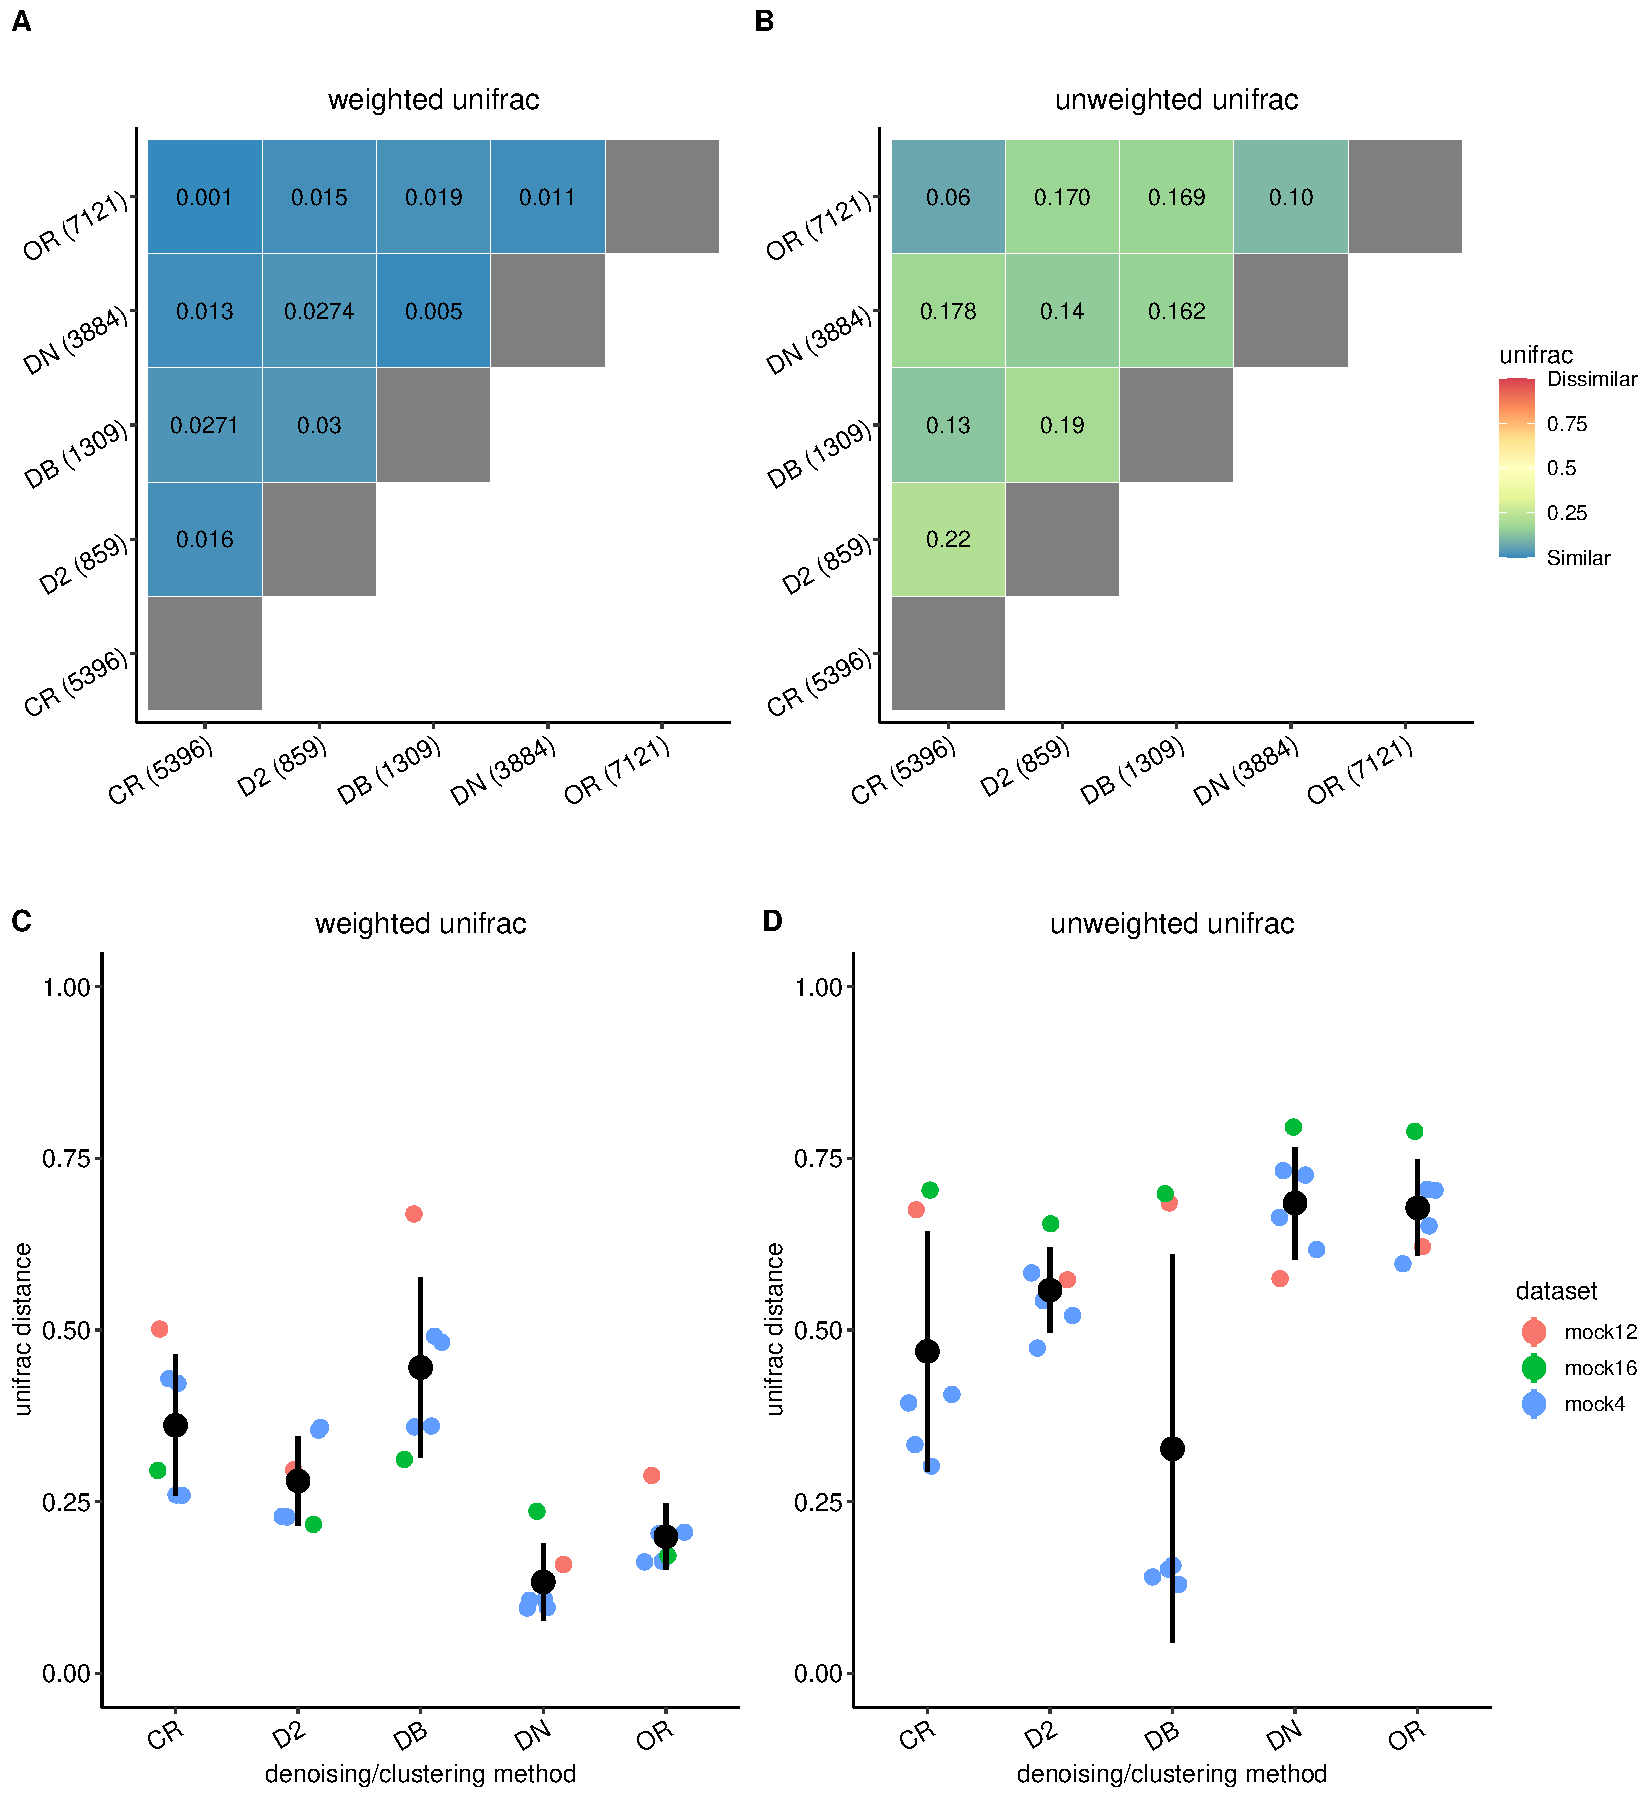
\includegraphics[width=\linewidth]{figure3.pdf}
  \caption{
    \textbf{Comparison of taxonomy assignments using different taxonomy reference databases}
    \textbf{(A)} Taxonomy composition of the 20 most abundant genera predicted using different taxonomy references databases: Greengenes, SILVA and NCBI.
    The legend shows the common and the unique genera among the taxonomy assignments.
    \textbf{(B)}
  }
  \label{fig:figure3}
\end{figure}

\begin{figure}[h]
  \centering
  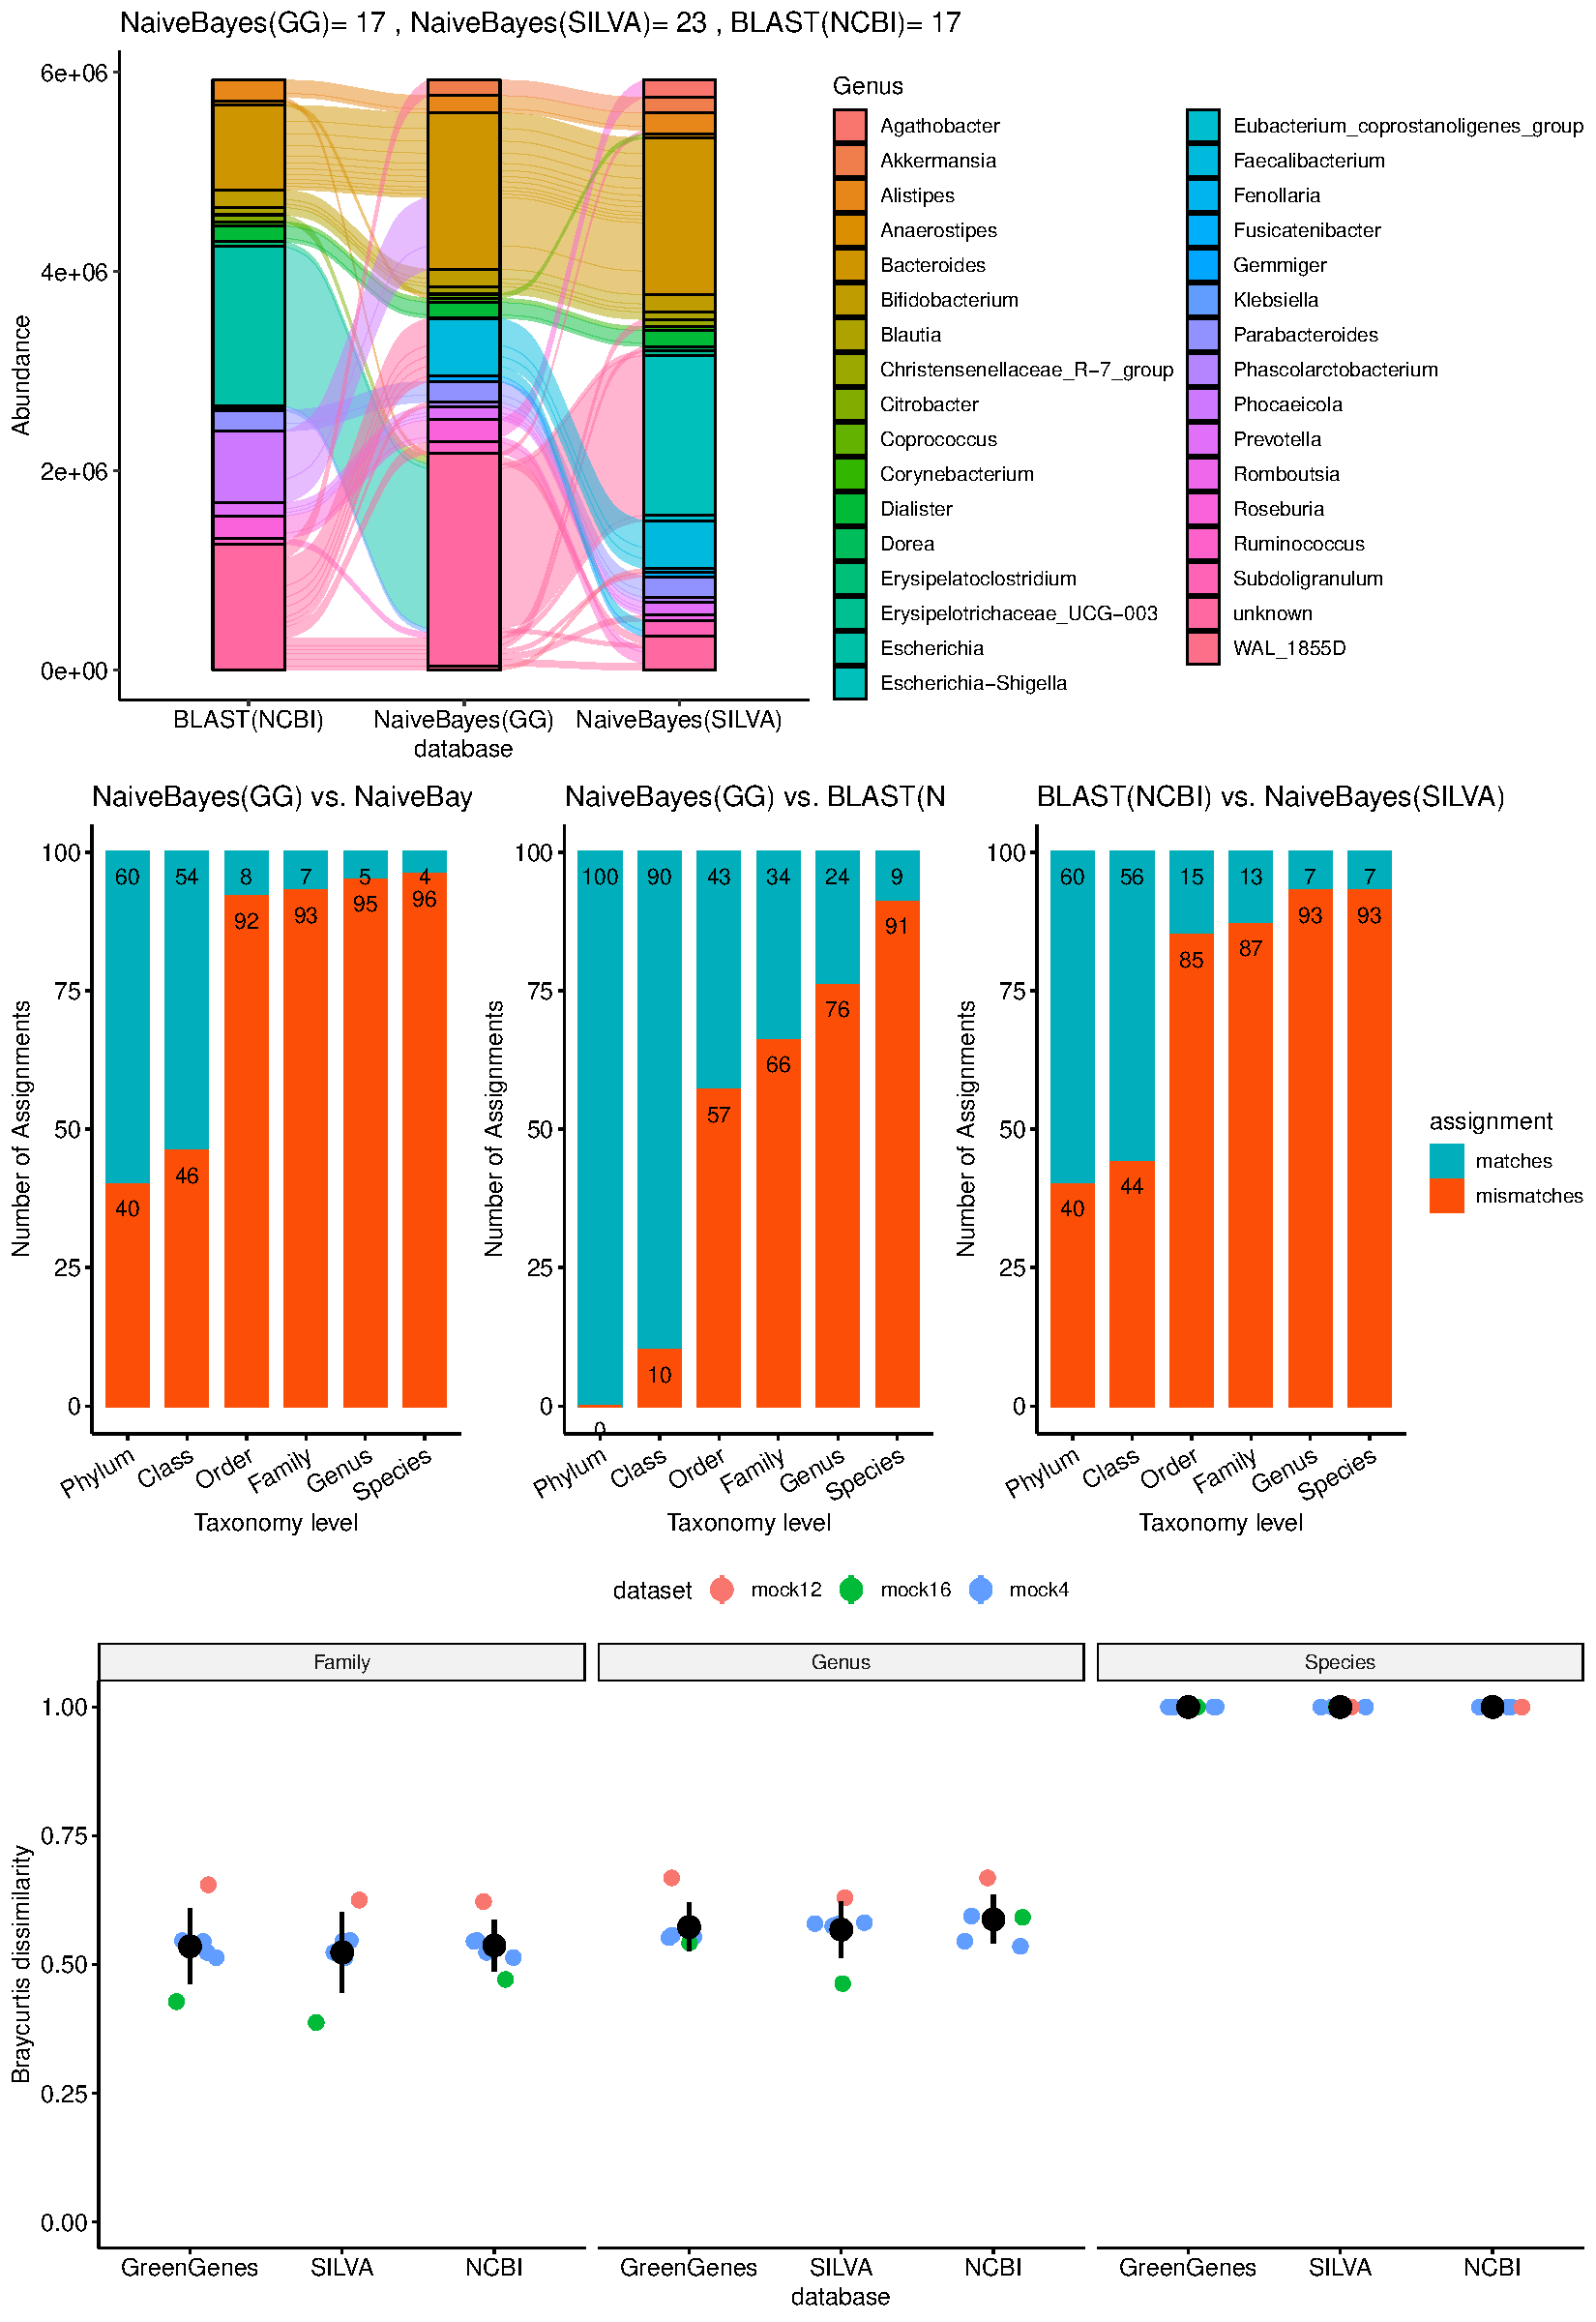
\includegraphics[width=\linewidth]{figure4.pdf}
  \caption{Effect of OTU processsing measures on the OTU table. This is just a placeholder}
  \label{fig:figure4}
\end{figure}

\begin{figure}[h]
  \centering
  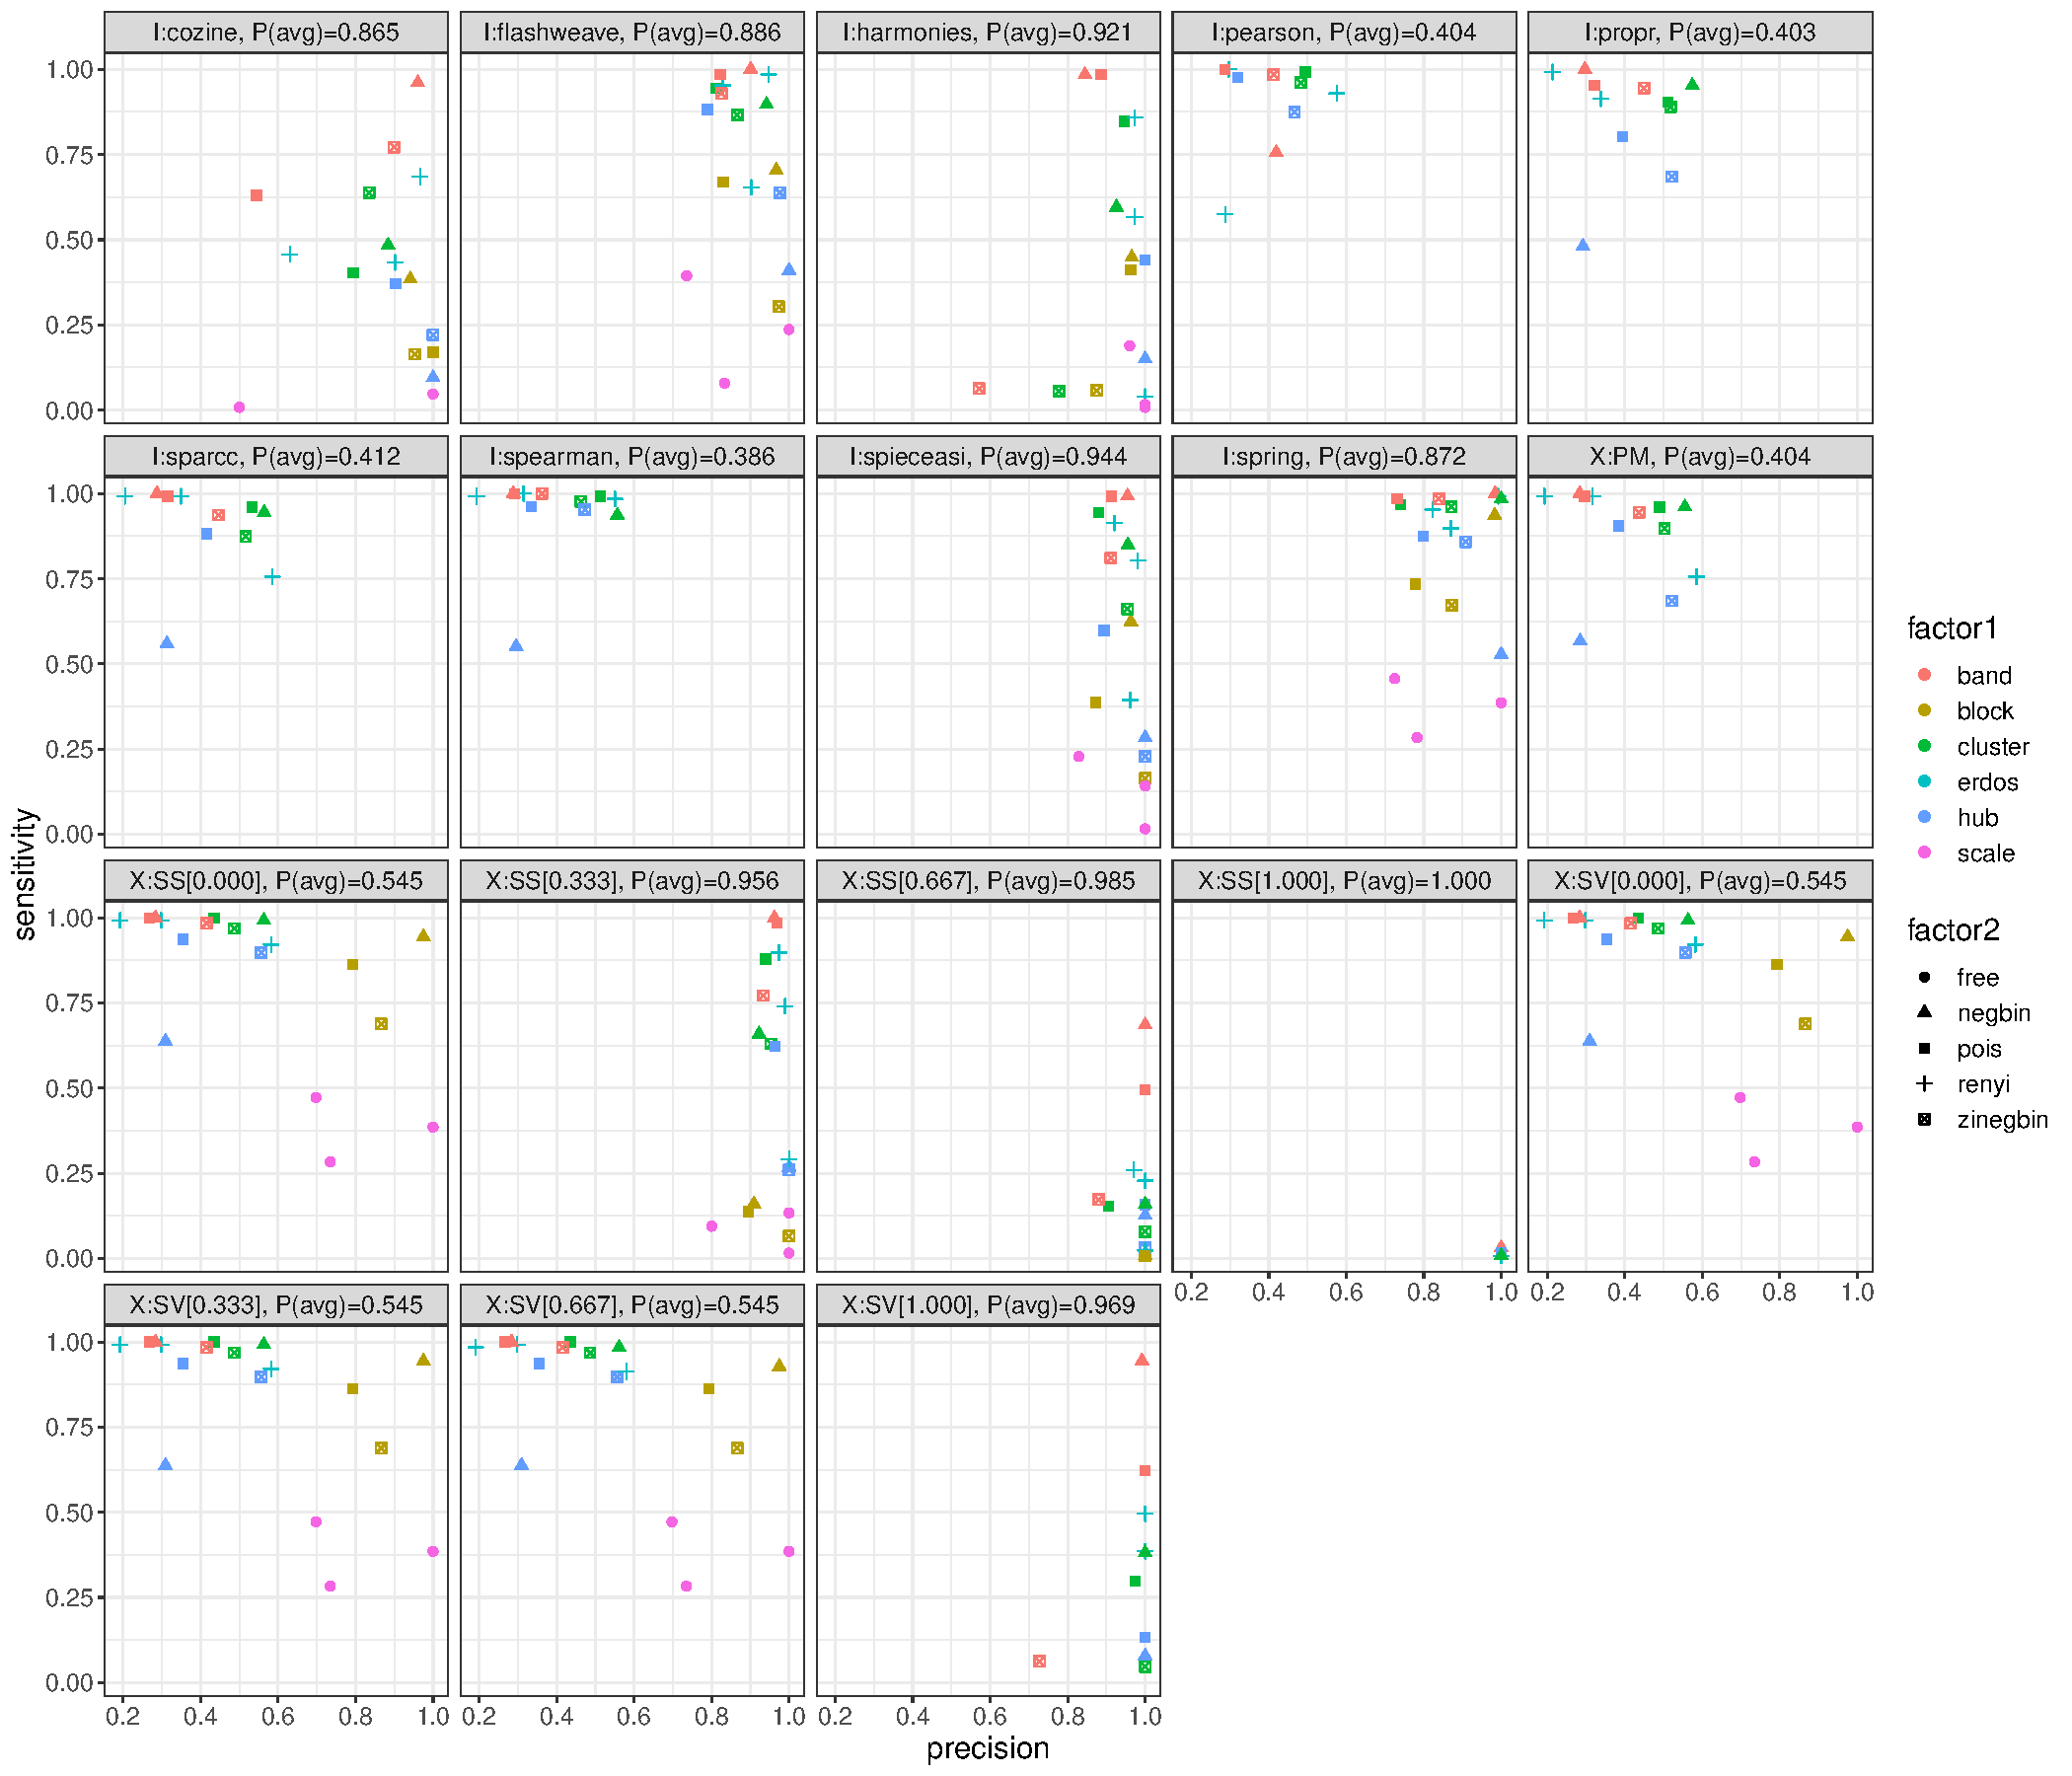
\includegraphics[width=\linewidth]{figure5.pdf}
  \caption{
    \textbf{Networks generated using different network inference methods}.
    The four different networks generated by different network inference methods are very dissimilar (C).
    (A) The overlaps between the edges among the network5 generated is shown. The number of edges that are common to all networks are very low (5).
    (B) The hamming distance between the networks is shown. The similarity between various methods was found to vary with the data-source used.
}
  \label{fig:figure5}
\end{figure}

\begin{figure}[h]
  \centering
  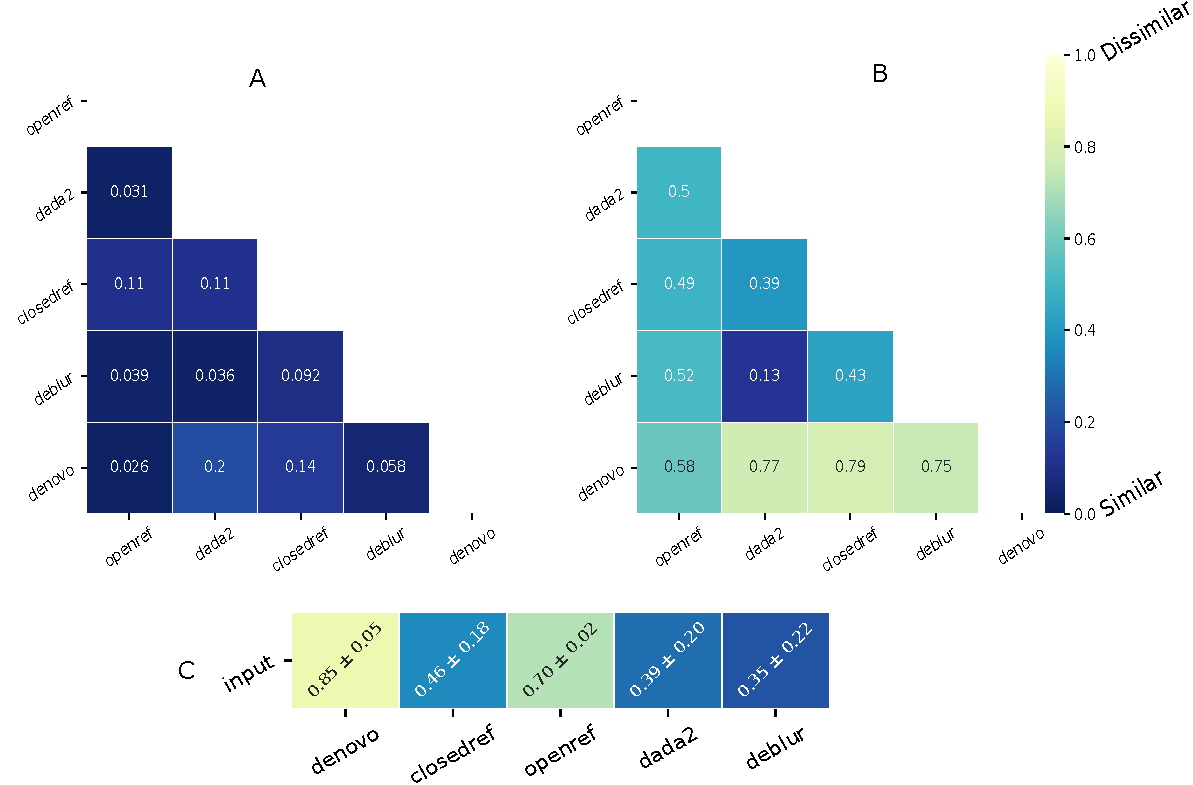
\includegraphics[width=\linewidth]{figure6.pdf}
  \caption{Example networks generated using our pipeline: Final consensus networks for some datasets}
  \label{fig:figure6}
\end{figure}

\FloatBarrier

\subsection*{Supplementary}%

\begin{figure}[h]
  \centering
  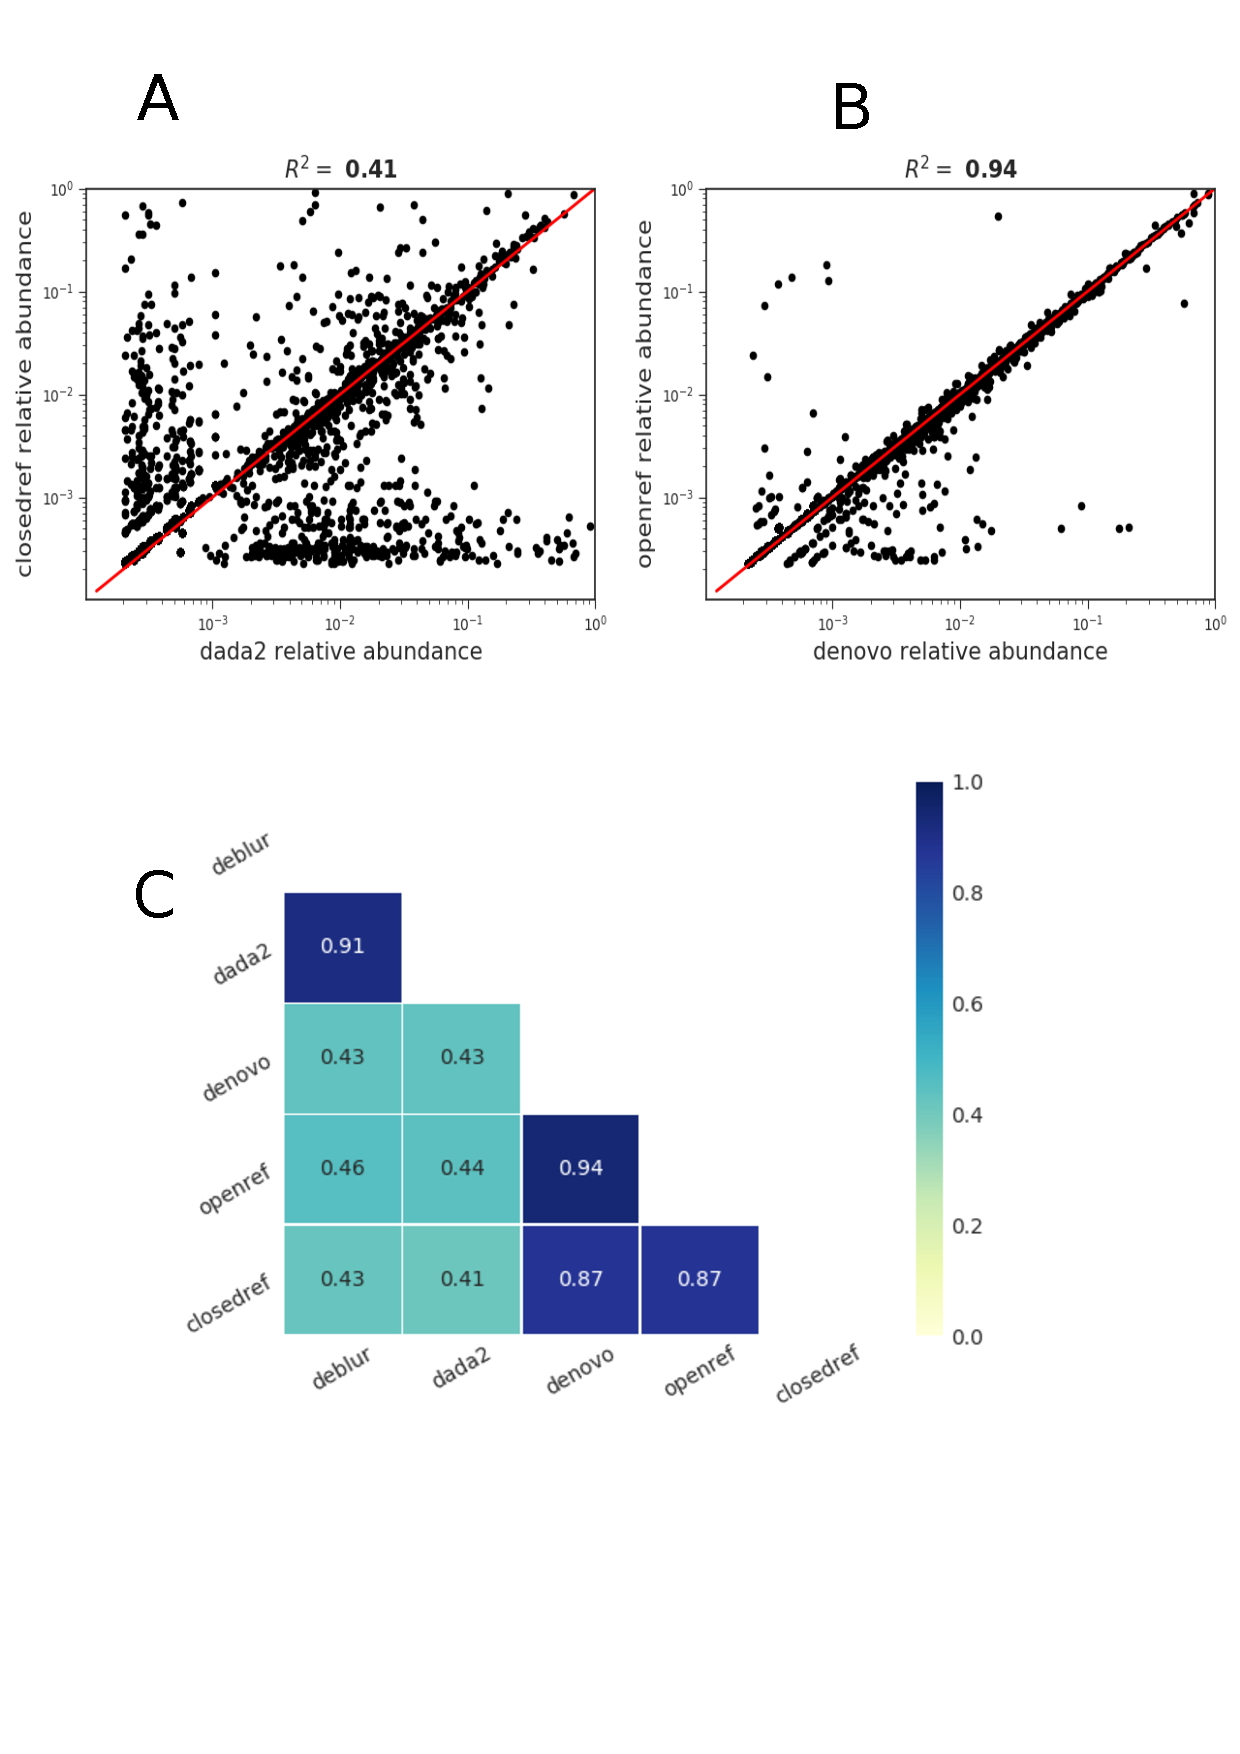
\includegraphics[width=0.67\linewidth]{figures1.pdf}
  \caption{
    \textbf{Comparison of various denoising and clustering algorithms used in the pipeline}.
    (A, B) Correlation of the abundances of the taxa that are common between the count matrices created by two different methods.
    (A) The best correlation (most similar methods) is between open-reference and denovo.
    (B) The worst correlation (least similar methods) is between open-reference and dada2.
    (C) A heatmap showing the $\mathrm{R}^2$ of all pairwise comparisons of the methods.
  }
  \label{fig:figures1}
\end{figure}

\begin{figure}[h]
  \centering
  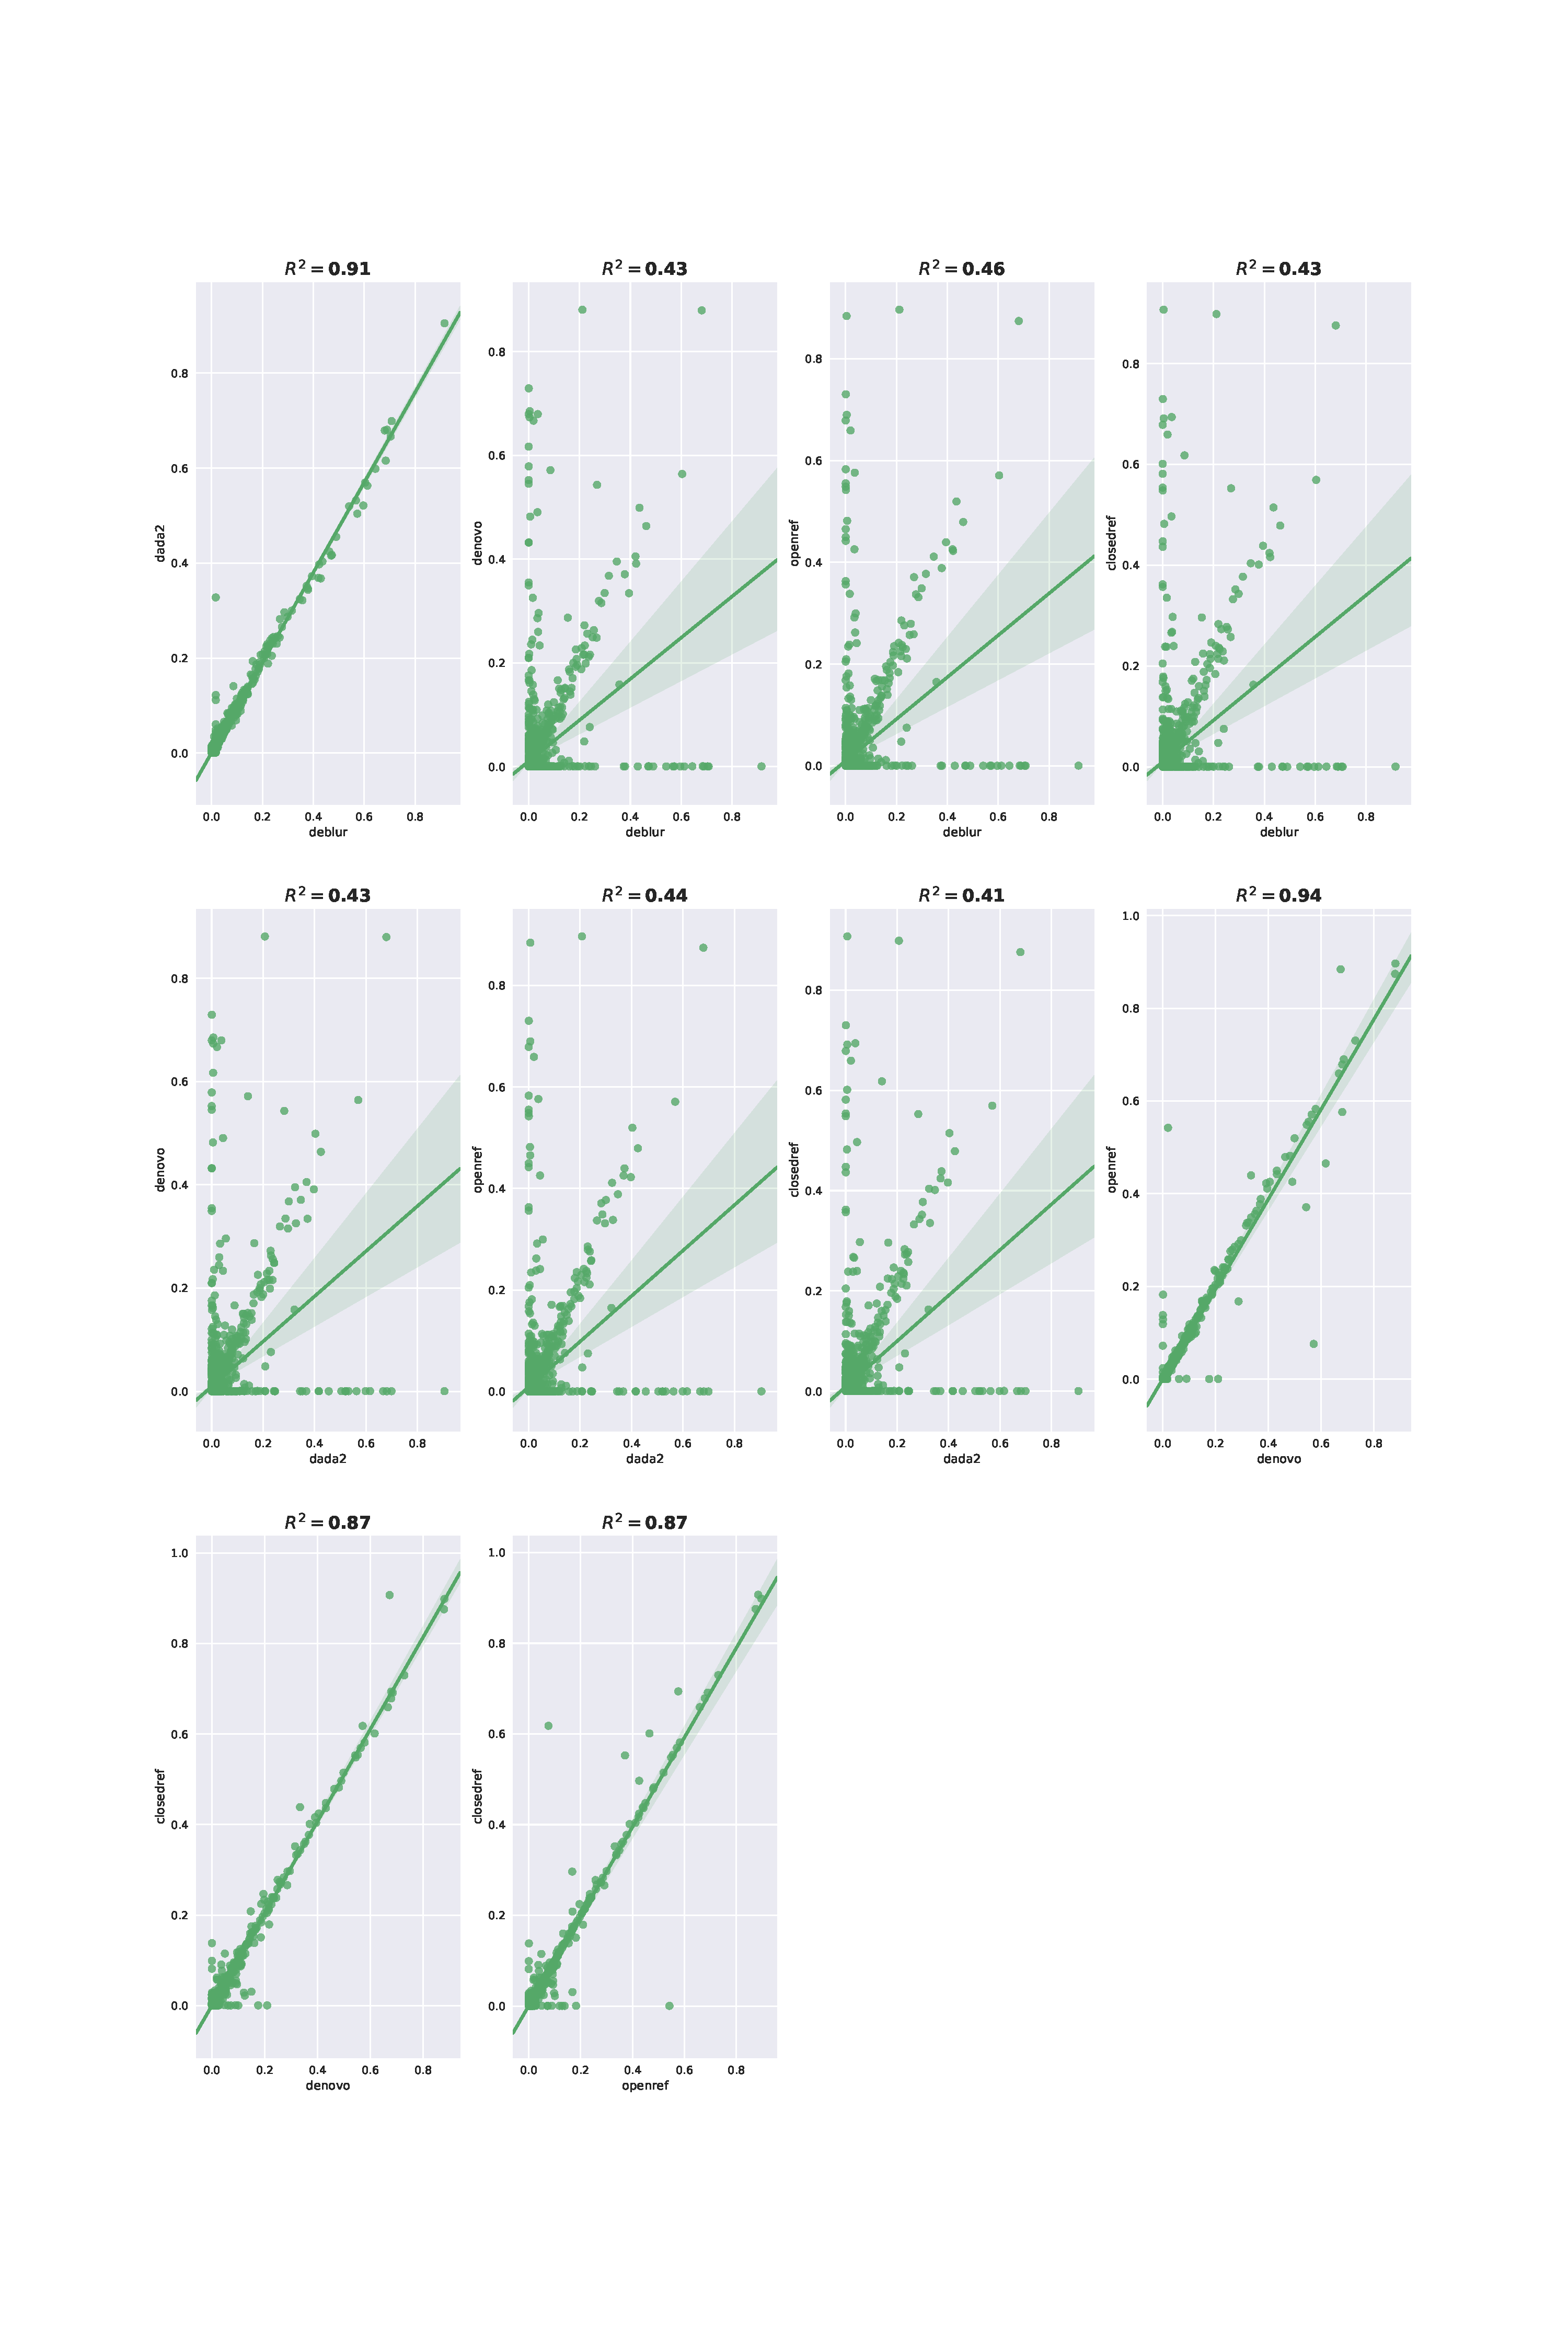
\includegraphics[width=0.8\linewidth]{pdf/all_denoise_reg.pdf}
  \caption{All pairwise correlations comparing the similarity between different denoising and clustering methods}
  \label{fig:figures2}
\end{figure}

\begin{figure}[h]
  \centering
  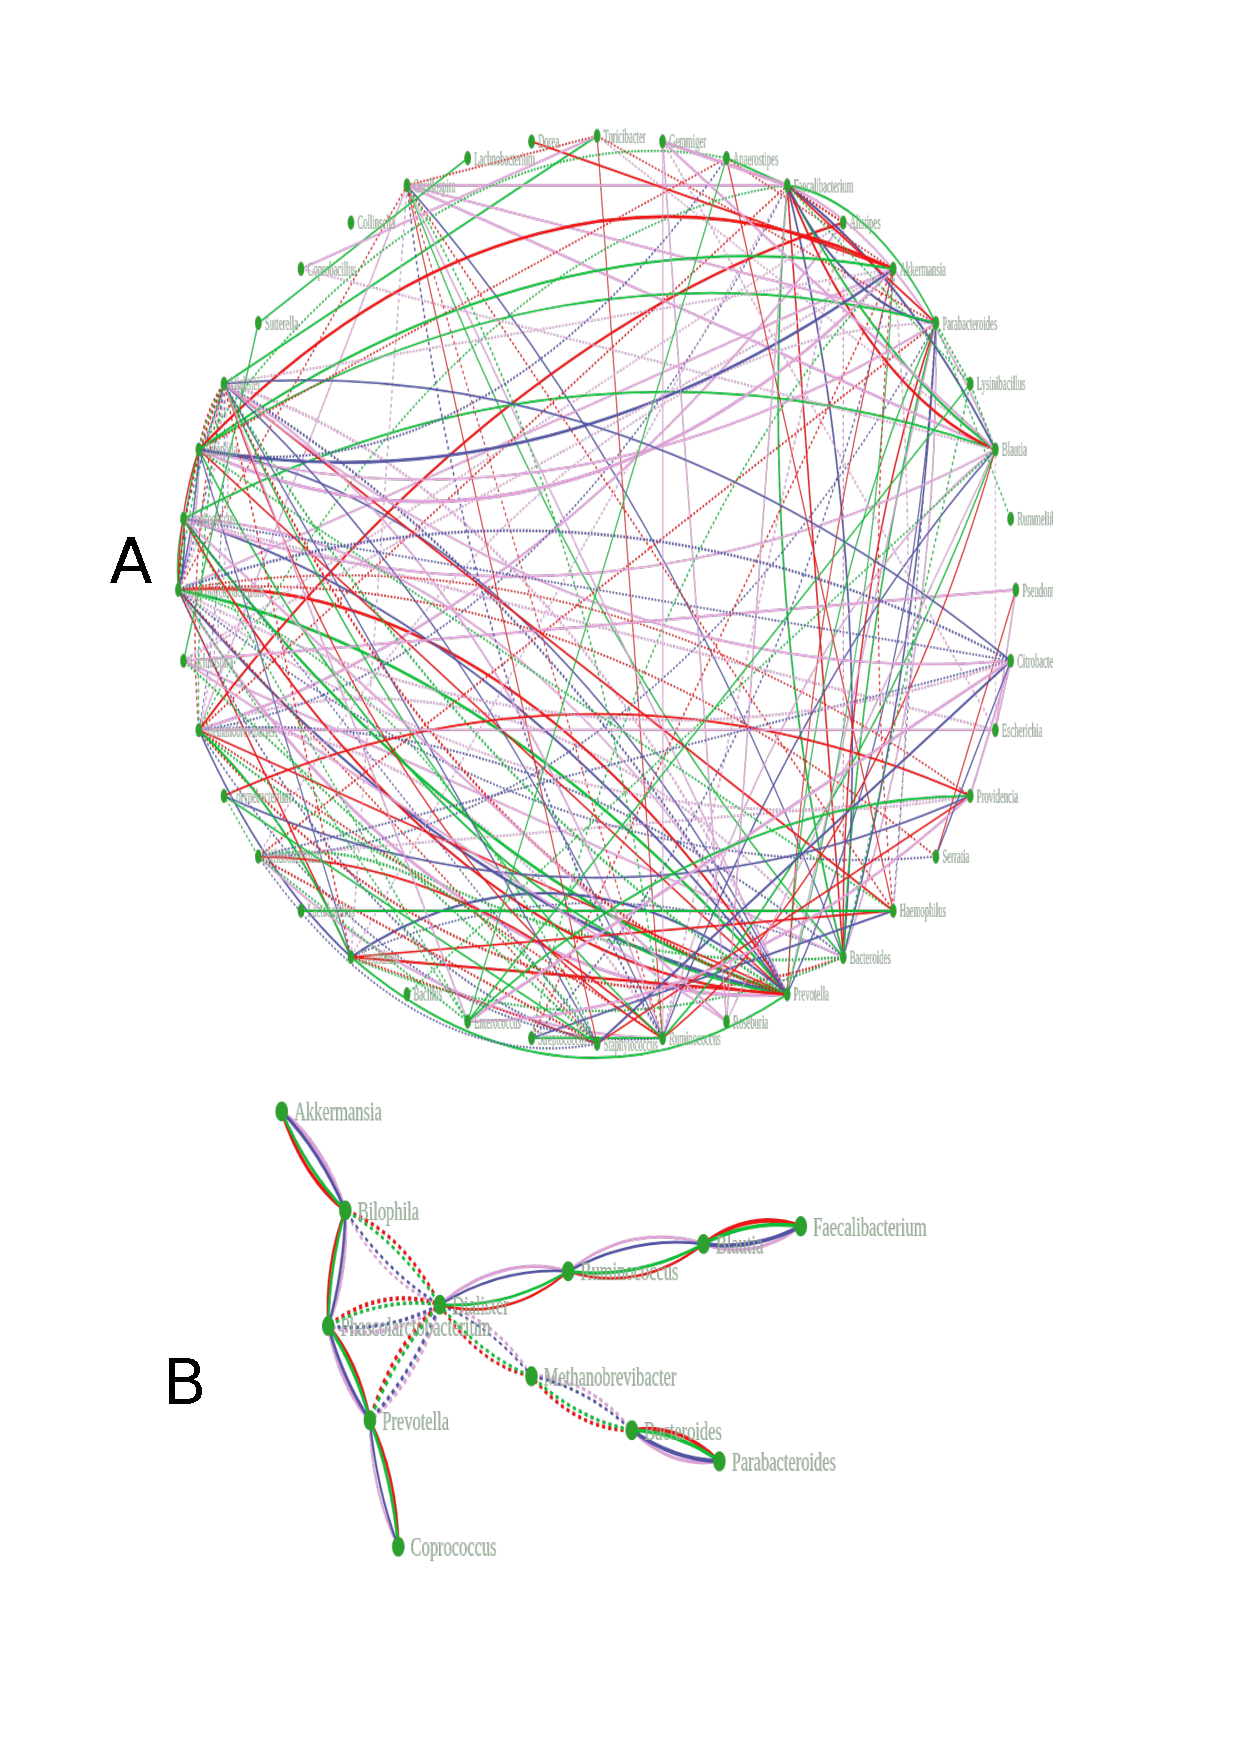
\includegraphics[width=0.8\linewidth]{pdf/denoise_network.pdf}
  \caption{A network showing union and intersection of networks generated using certain combination of methods}
  \label{fig:pdf/denoise_network}
\end{figure}



\end{document}
